\documentclass[crop,tikz,border=2px]{standalone}
\usepackage{tikzsymbols}
\usetikzlibrary{arrows,positioning,scopes}
\begin{document}
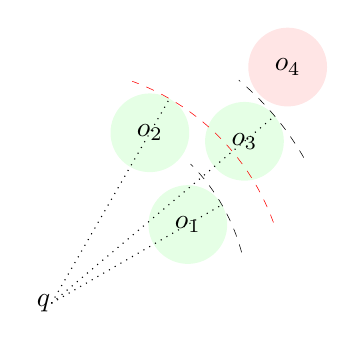
\begin{tikzpicture}[
  ur/.style={circle,minimum width=1cm,node distance=.5cm},
  cand/.style={fill=green!10},
  noncand/.style={fill=red!10},
  bound/.style={very thin,dashed},
  dist/.style={thin,dotted}]

  \node[ur,cand] (r1) at ([shift=(30:2cm)]0,0) {\(o_1\)};
  \node[ur,cand] (r2) at ([shift=(60:2.5cm)]0,0) {\(o_2\)};
  \node[ur,cand] (r3) at ([shift=(40:3.2cm)]0,0) {\(o_3\)};
  \node[ur,noncand] (r4) at (3,3) {\(o_4\)};

  \draw[dist] (0,0) -- ++(30:2.5cm);
  \draw[dist] (0,0) -- ++(60:3cm);
  \draw[dist] (0,0) -- ++(40:3.7cm);

  \draw[bound] ([shift=(15:2.5cm)]0,0) arc (15:45:2.5cm);
  \draw[bound,red] ([shift=(20:3cm)]0,0) arc (20:70:3cm);
  \draw[bound] ([shift=(30:3.7cm)]0,0) arc (30:50:3.7cm);

  \node at (-.1,0) {\(q\)};
\end{tikzpicture}
\end{document}